\documentclass[12pt, twoside]{article}
\documentclass[12pt, twoside]{article}
\usepackage[letterpaper, margin=1in, headsep=0.2in]{geometry}
\setlength{\headheight}{0.6in}
%\usepackage[english]{babel}
\usepackage[utf8]{inputenc}
\usepackage{microtype}
\usepackage{amsmath}
\usepackage{amssymb}
%\usepackage{amsfonts}
\usepackage{siunitx} %units in math. eg 20\milli\meter
\usepackage{yhmath} % for arcs, overparenth command
\usepackage{tikz} %graphics
\usetikzlibrary{quotes, angles}
\usepackage{graphicx} %consider setting \graphicspath{{images/}}
\usepackage{parskip} %no paragraph indent
\usepackage{enumitem}
\usepackage{multicol}
\usepackage{venndiagram}

\usepackage{fancyhdr}
\pagestyle{fancy}
\fancyhf{}
\renewcommand{\headrulewidth}{0pt} % disable the underline of the header
\raggedbottom
\hfuzz=2mm %suppresses overfull box warnings

\usepackage{hyperref}

\fancyhead[LE]{\thepage}
\fancyhead[RO]{\thepage \\ Name: \hspace{4cm} \,\\}
\fancyhead[LO]{BECA / Dr. Huson / Geometry\\*  Unit 10: Similarity and proportions \\* 31 March 2023}

\begin{document}

\subsubsection*{9.10 Classwork: Similarity transformations}
I can solve problems using similarity criteria. \hfill CCSS.HSG.SRT.B.5
\begin{enumerate}
\begin{multicols}{2}
[\item A dilation maps triangle $PQR$ onto triangle $STU$ with $QR=6$ and $TU=12$.] %\vspace{1cm}
  \begin{enumerate}
    \item $\overline{PR} \rightarrow$ \rule{2cm}{0.15mm}
    \item What scale factor maps\\
      $\triangle PQR \rightarrow \triangle STU$? \vspace{0.75cm}
    \item Given $PR=8$, find $SU$. \vspace{0.75cm}
    \item Given $ST=6$, find $PQ$.
    \end{enumerate}
    \begin{tikzpicture}[scale=0.7]
      \coordinate [label=above left:$P$](A) at (85:2);
      \coordinate [label=below:$Q$](B) at (0, 0);
      \coordinate [label=right:$R$](C) at (-20:3);
      \draw [thick] (A)--(B)--(C)--cycle;
      \draw [thick, xshift=2cm, yshift=2.5cm] (85:4) node[above]{$S$}--
      (0,0) node[below]{$T$}--
      (-20:6) node[right]{$U$}--cycle;
    \end{tikzpicture}
  \end{multicols}  \vspace{2cm}

\item Given $\triangle ABC \sim \triangle DEF$, $m\angle A=55^\circ$, and $m\angle B=95^\circ$. Find $m\angle E$. \vspace{2.5cm}

\item Triangle $ABC$ is dilated with a scale factor of $k$ centered at $A$, yielding $\triangle ADE$, as shown. Given $AB=10$, $BC=14$, $AC=16$, and $DE=21$.
\begin{multicols}{2}
  \begin{enumerate}[itemsep=1.5cm]
    \item Find the scale factor, $k$
    \item Find $AD$
    \item Find $CE$
  \end{enumerate}
  \begin{center}
    \begin{tikzpicture}[scale=0.6]
      \draw [thick]
      (0,0)node[left]{$B$}--
      (8,0)node[above right]{$C$}--
      (2,6)node[left]{$A$}--cycle;
      \draw [thick]
      (0,0)--
      (-1,-3)node[left]{$D$}--
      (11,-3)node[above right]{$E$}--(8,0);
      \node at (4,0)[below]{$14$};
      \node at (5.3, 3)[right]{$16$};
      \node at (0.3, 2.8)[above]{$10$};
      \node at (5,-3)[below]{$21$};
    \end{tikzpicture}
  \end{center}
\end{multicols}
\vspace{1cm}

\newpage
\item Dilate $\triangle JKL$ with a scale factor $k=2$ centered on the origin. Draw the image $\triangle J'K'L'$ and label its vertices. Given $J(-3,-2)$, $K(3,-2)$, and $L(0,3)$.
  \begin{center}
    \begin{tikzpicture}[scale=.7]
      \draw [help lines] (-8,-6) grid (8,8);
      \draw [thick, <->] (-8.4,0) -- (8.4,0) node [right] {$x$};
      \draw [thick, ->] (0,-6)--(0,8.4) node [right] {$y$};
      \draw [thick]
      (-3,-2) node[below] {$J$}--
      (3,-2) node[below] {$K$}--
      (0,3) node[above right] {$L$}--cycle;
    \end{tikzpicture}
  \end{center}

\item In the diagram below, $\angle ABC \cong \angle ADE$, $AB = 7$, $AC = 6$, $BD = 14$, and $DE = 15$. Find  $AD$ and the scale factor $k$. Then find $AE$ and $BC$. %\vspace{1cm}
\begin{multicols}{2}
  \begin{enumerate}[itemsep=1.25cm]
    \item $AD=$
    \item $k=$
    \item $AE=$
    \item $BC=$
  \end{enumerate}
  \begin{flushright}
    \begin{tikzpicture}[scale=0.8]
      \draw [-, thick] (0,0) node[above left]{$A$}--
      (8,0) node[below]{$E$}--
      (9,6) node[above left]{$D$}--cycle;
      \draw [thick] (3.2,0)--(3.6,2.4);
      \node at (3.5,0) [below]{$C$};
      \node at (4,2.7) [above left]{$B$};
      \node at (2, 0) [below]{$6$};
      \node at (1.8,1.5) [above]{$7$};
      \node at (8.5, 3) [right]{$15$};
      \node at (5.1, 4.5) [right]{$14$}; \vspace{1cm}
    \end{tikzpicture}
  \end{flushright} 
\end{multicols}\vspace{1cm}

\newpage
\item Given $\triangle ABP$ and $\triangle JKP$ as shown below. $\overline{AB} \parallel \overline{JK}$. $AP=7.36$, $JP=16.56$, and $JK=18.9$. Find $AB$.
\begin{flushright}
  \begin{tikzpicture}[scale=1.4]
      \draw [thick]
        (0.25,-1)node[right]{$B$}--
        (-0.5,2)node[left]{$K$}--
        (4,0)node[right]{$J$}--
        (0,0)node[above right]{$P$}--
        (-2,0)node[left]{$A$}--cycle;
    \end{tikzpicture}
    \end{flushright}
\vspace{1cm}

\item The line $\overleftrightarrow{AB}$ has the equation $y=\frac{3}{2}x-3$. Apply a dilation mapping $\overleftrightarrow{AB} \rightarrow \overleftrightarrow{A'B'}$ with a factor of $k=2$ centered at the origin. Draw and label the image on the grid. Write the equation of the line $\overleftrightarrow{A'B'}$.
  \begin{flushright} %4 quadrant regents grid w T-Chart
  \begin{tikzpicture}[scale=.635]
    \draw [help lines] (-1,-7) grid (10,1);
    \draw [thick, ->] (-1.2,0) -- (10.4,0) node [below right] {$x$};
    \draw [thick, ->] (0,-7.2)--(0,1.4) node [left] {$y$};
    \draw [<->, thick] (-0.5,-3.75)--(2.5,0.75);
    \draw [fill] (0,-3) circle [radius=0.1]node[above left]{$A$};
    %\draw [fill] (3,0) circle [radius=0.1]node[below left]{$C$};
    \draw [fill] (2,0) circle [radius=0.1]node[below right]{$B$};
  \end{tikzpicture}
  \end{flushright}

\item What is the smallest non-zero angle of rotation about its center that would map the pentagon onto itself? \vspace{0.25cm} %$ABCDE$
  \begin{center}
      \begin{tikzpicture}%[scale=.48]
        \draw [thick]
        (0:2)--% node[right] {$A$}--
        (72:2)--% node[above right] {$B$}--
        (144:2)--% node[above left] {$C$} --
        (216:2)--% node[left] {$D$}--
        (288:2)--cycle;% node[right] {$E$}--cycle;
      \end{tikzpicture}
    \end{center} \vspace{0.5cm}

\newpage
\begin{multicols}{2}[\item The diagram below shows $\triangle ABC$, with $\overline{AEB}$, $\overline{ADC}$, and $\angle ACB \cong \angle AED$. $AB=14$, $AD=8$, and $DE=4$.]
  \begin{enumerate}
    \item $\overline{AE} \rightarrow$ \rule{2cm}{0.15mm} \vspace{0.5cm}
    \item $\overline{AD} \rightarrow$ \rule{2cm}{0.15mm} \vspace{0.5cm}
    \item $\triangle ADE \sim$ \rule{2cm}{0.15mm} \vspace{0.5cm}
    \item What is the scale factor?\\[0.5cm] $k=$  \rule{2cm}{0.15mm}
    \item What is the length of $\overline{BC}$?
  \end{enumerate}
    \begin{tikzpicture}[scale=1.2]
      \draw [thick]
      (0,0) node[above right] {$A$}--
      (230:6) node[below left] {$B$}--
      (260:4.75) node[below right] {$C$}--cycle;
      \draw [thick]
      (230:2.375) node[above left] {$E$}--
      (260:3) node[right] {$D$}--cycle;
    \end{tikzpicture}
  \end{multicols} \vspace{2cm}

\item Triangle $ADE$ and its midline $\overline{BC}$ are drawn, with $B$ the midpoint of $\overline{AD}$ and $C$ the midpoint of $\overline{AE}$. The two medians $\overline{BE}$ and $\overline{CD}$ are drawn, as shown, intersecting in point $F$, the centroid. Given $BC=8$, $FE=10$.
\begin{multicols}{2}
  \begin{enumerate}[itemsep=1.5cm]
    \item Write down $DE$.
    \item Given $\triangle FCB \sim \triangle FDE$ with scale factor $k=2$. \\[0.5cm]
     Find $BF$.
     \item Given the area of $\triangle FCB = 12.5$, find the area of $\triangle FDE$.
  \end{enumerate}
  \begin{center}
    \begin{tikzpicture}[scale=0.55]
      \draw [thick]
      (0.5,1.5)node[left]{$B$}--
      (6.5,1.5)node[above right]{$C$}--
      (2,6)node[above]{$A$}--cycle;
      \draw [thick]
      (0.5,1.5)--
      (-1,-3)node[left]{$D$}--
      (11,-3)node[above right]{$E$}--(6.5,1.5);
      \draw [thick] (0.5,1.5)--(11,-3);
      \draw [thick] (6.5,1.5)--(-1,-3);
      \node at (3,2.5)[below]{$8$};
      \node at (3.5, -0.6)[right]{$F$};
      \node at (6.6, -.9)[above]{$10$};
      %\node at (-0.7, -1)[above]{$5$};
    \end{tikzpicture}
  \end{center}
\end{multicols}
 \vspace{1cm}

\newpage
\item In the diagram below, the chords $\overline{AE}$ and $\overline{BD}$ intersect at $C$, with $\triangle ABC \sim \triangle DEC$, $BC=3.4$, $AC=4.2$, and $BD=9.35$. Determine the length of $\overline{CE}$.
    \begin{center}
    \begin{tikzpicture}[scale=.6]
      \draw (0,0) circle[radius=5];
      \draw [thick]
      (20:5) node[right] {$A$}--
      (160:5) node[left] {$E$}--
      (210:5) node[left] {$D$}--
      (50:5) node[above right] {$B$}--cycle;
      \draw (75:1.8) node[above] {$C$};
    \end{tikzpicture}
  \end{center} \vspace{2cm}

\item In the diagram below $\triangle ABC \sim \triangle DEF$, $DE=10$, $AB=x$, $AC=3x$, $DF=2x+14$. \\[0.25cm] 
Determine the length of $\overline{AB}$.
  \begin{center}
    \begin{tikzpicture}[scale=1]
    \coordinate [label=above left:$A$](A) at (85:2);
    \coordinate [label=below:$B$](B) at (0, 0);
    \coordinate [label=right:$C$](C) at (-20:3);
      \draw [thick] (A)--(B)--(C)--cycle;
      \node at (95:1)[left]{$x$};
      \node at (35:1.75)[right]{$3x$};
      \draw [thick, xshift=5cm, yshift=0.5cm] (85:3) node[above]{$D$}--
      (0,0) node[below]{$E$}--
      (-20:4.5) node[right]{$F$}--cycle;
      \draw [thick, xshift=5cm, yshift=0.5cm](90:1.5) node[left]{$10$};
      \draw [thick, xshift=5cm, yshift=0.5cm](30:2.75) node[right]{$2x+14$};
  \end{tikzpicture}
  \end{center}

\newpage
\item In triangle $ABC$, points $D$ and $E$ are on sides of $\overline{AB}$ and $\overline{BC}$, respectively, such that $\overline{DE} \parallel \overline{AC}$, and $BD:DA = 5:3$.\\[0.5cm]
If $DB=9.0$ and $DE=10.5$, what is the length of $\overline{AC}$, to the \emph{nearest tenth}?
\begin{flushright}
  \begin{tikzpicture}[scale=0.5, rotate=-11]
    \draw [thick]
    (0,0)node[above]{$B$}--
    (-130:10)node[below]{$A$}--
    (-40:8)node[below]{$C$}--cycle;
    \draw [thick]
    (-130:6)node[above left]{$D$}--
    (-40:4.8)node[right]{$E$};
  \end{tikzpicture}
\end{flushright} \vspace{2cm}

\item In the diagram below $\triangle ABC \sim \triangle DEF$, $DE=x$, $AB=3$, $AC=x-1$, $DF=x+7$. \\[0.25cm] 
Find $x$.
  \begin{center}
    \begin{tikzpicture}[scale=1]
    \coordinate [label=above left:$A$](A) at (85:2);
    \coordinate [label=below:$B$](B) at (0, 0);
    \coordinate [label=right:$C$](C) at (-20:3);
      \draw [thick] (A)--(B)--(C)--cycle;
      \node at (95:1)[left]{$3$};
      \node at (35:1.75)[right]{$x-1$};
      \draw [thick, xshift=5cm, yshift=0.5cm] (85:3) node[above]{$D$}--
      (0,0) node[below]{$E$}--
      (-20:4.5) node[right]{$F$}--cycle;
      \draw [thick, xshift=5cm, yshift=0.5cm](90:1.5) node[left]{$x$};
      \draw [thick, xshift=5cm, yshift=0.5cm](30:2.75) node[right]{$x+7$};
  \end{tikzpicture}
  \end{center}

\end{enumerate}
\end{document}
